\chapter{General Project Presentation}

\section{Introduction}
This introductory chapter establishes the foundational context of this graduation project. We begin by introducing the host organization, HMI Stars Consulting, outlining its operational structure and the administrative consulting ecosystem in which it operates. We then detail the core problem statement, highlighting the challenges of manual workflows in client-consultant coordination, followed by the proposed digital solution. Finally, this chapter outlines our methodological framework—the Two-Track Unified Process (2TUP)—and presents a comparative analysis of existing enterprise resource planning (ERP) platforms to substantiate our subsequent architectural and technology selections.

\section{Company presentation}
The internship was conducted remotely at \textbf{HMI Stars Consulting}, a consulting company specialized in project management, company registration, and social and tax administrative support.
The company offers services such as helping clients draft legal statutes and manage daily administrative tasks, including social declarations, employment contract tracking, salary processing, and communication with public authorities.
HMI Stars Consulting works with small and medium-sized enterprises (SMEs) based in France. To ensure proper follow-up, it relies on administrative staff, including secretaries and administrators, who work closely with client company managers.
\begin{figure}[H]
    \centering
    
\includegraphics[width=0.35\linewidth]{images/hmi_stars.jpeg}
    \caption{HMI Stars logo}
    \label{fig:HMI Stars logo}
\end{figure}

\section{Preliminary Study}

\subsection{Study of the existing}

\subsubsection{Description of the existing}
To find a solution to our problem, we conducted research on existing systems. We chose three platforms that offer business administration, client portals, and document management capabilities:
\begin{itemize}
    \item \textbf{Odoo (Community Edition)}:
    Odoo is an open-source business software suite offering a range of integrated applications for various business needs. It includes modules for accounting, customer relationship management (CRM), human resources, and document sharing. It allows client companies to upload records through web forms, although customizing portal views and real-time interaction flows requires advanced technical setups.
    \begin{figure}[H]
        \centering
        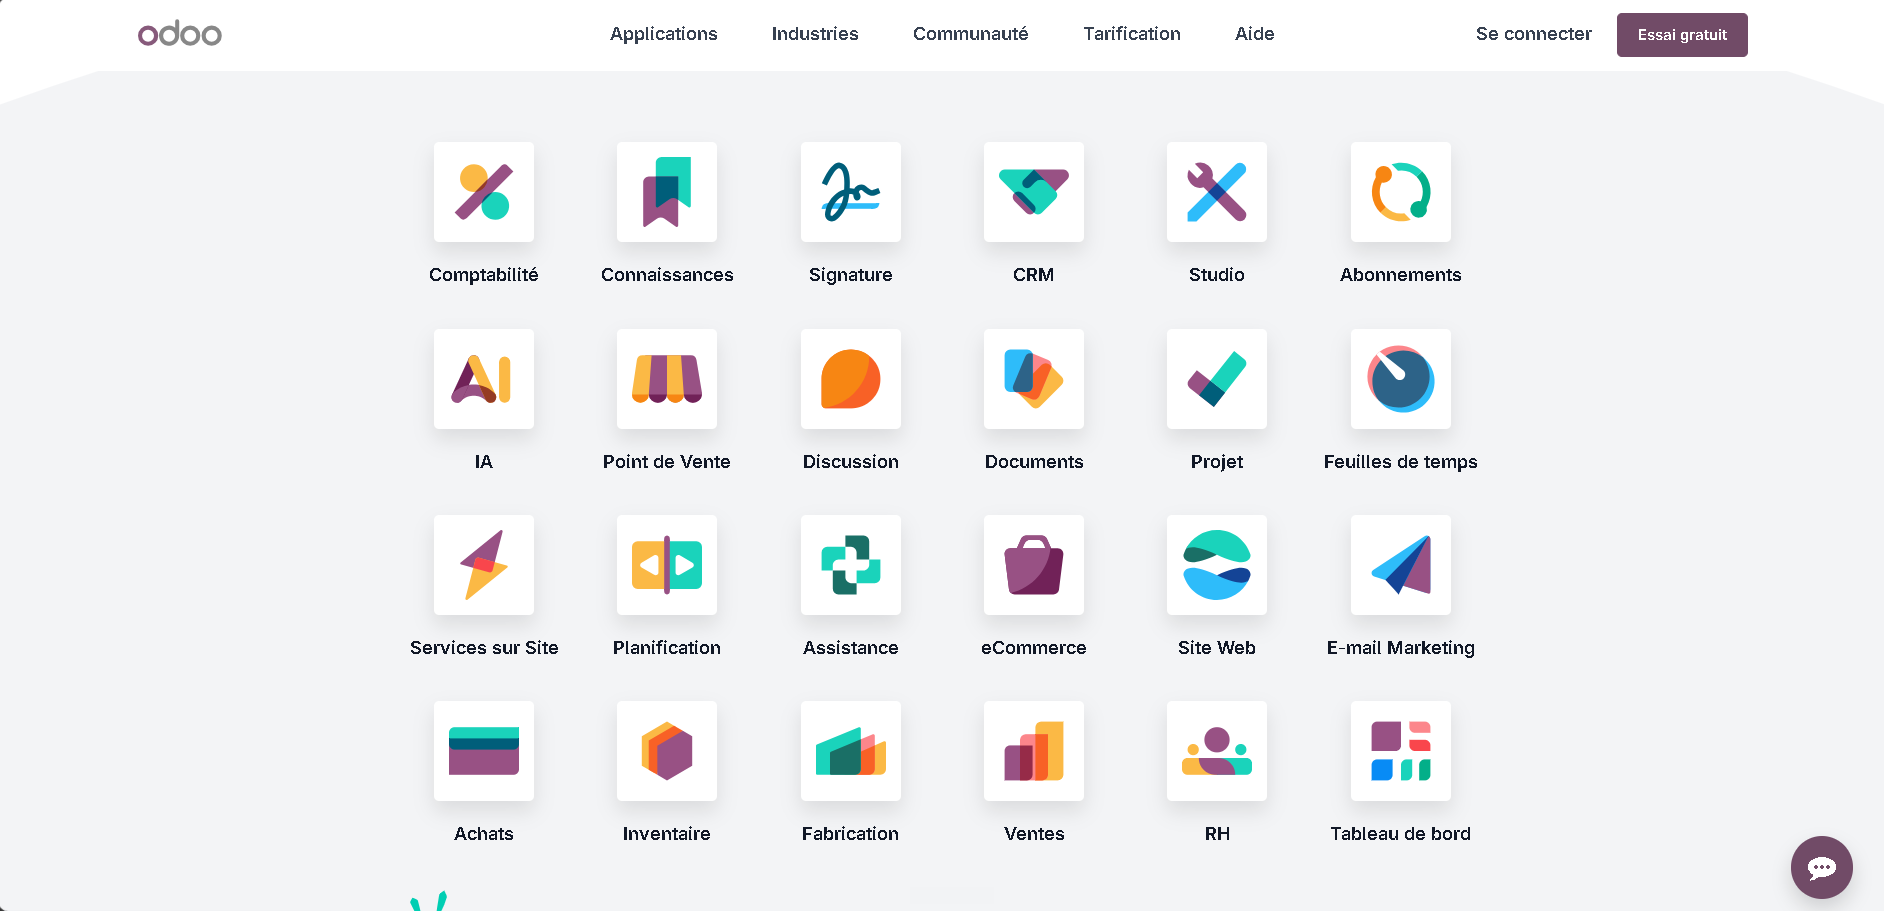
\includegraphics[width=1\linewidth]{images/odoo.png}
        \caption{Odoo Logo}
        \label{fig:Odoo Logo}
    \end{figure}
    
    \item \textbf{ERPNext}:
    ERPNext is an open-source Enterprise Resource Planning (ERP) platform built on the Frappe framework. It is designed for small and medium-sized enterprises and includes features such as client portals, employee directory management, expense tracking, and support ticket systems.
    However, its messaging system does not provide real-time synchronization by default, and it does not include a dedicated mobile application for clients.
        \begin{figure}[H]
        \centering
        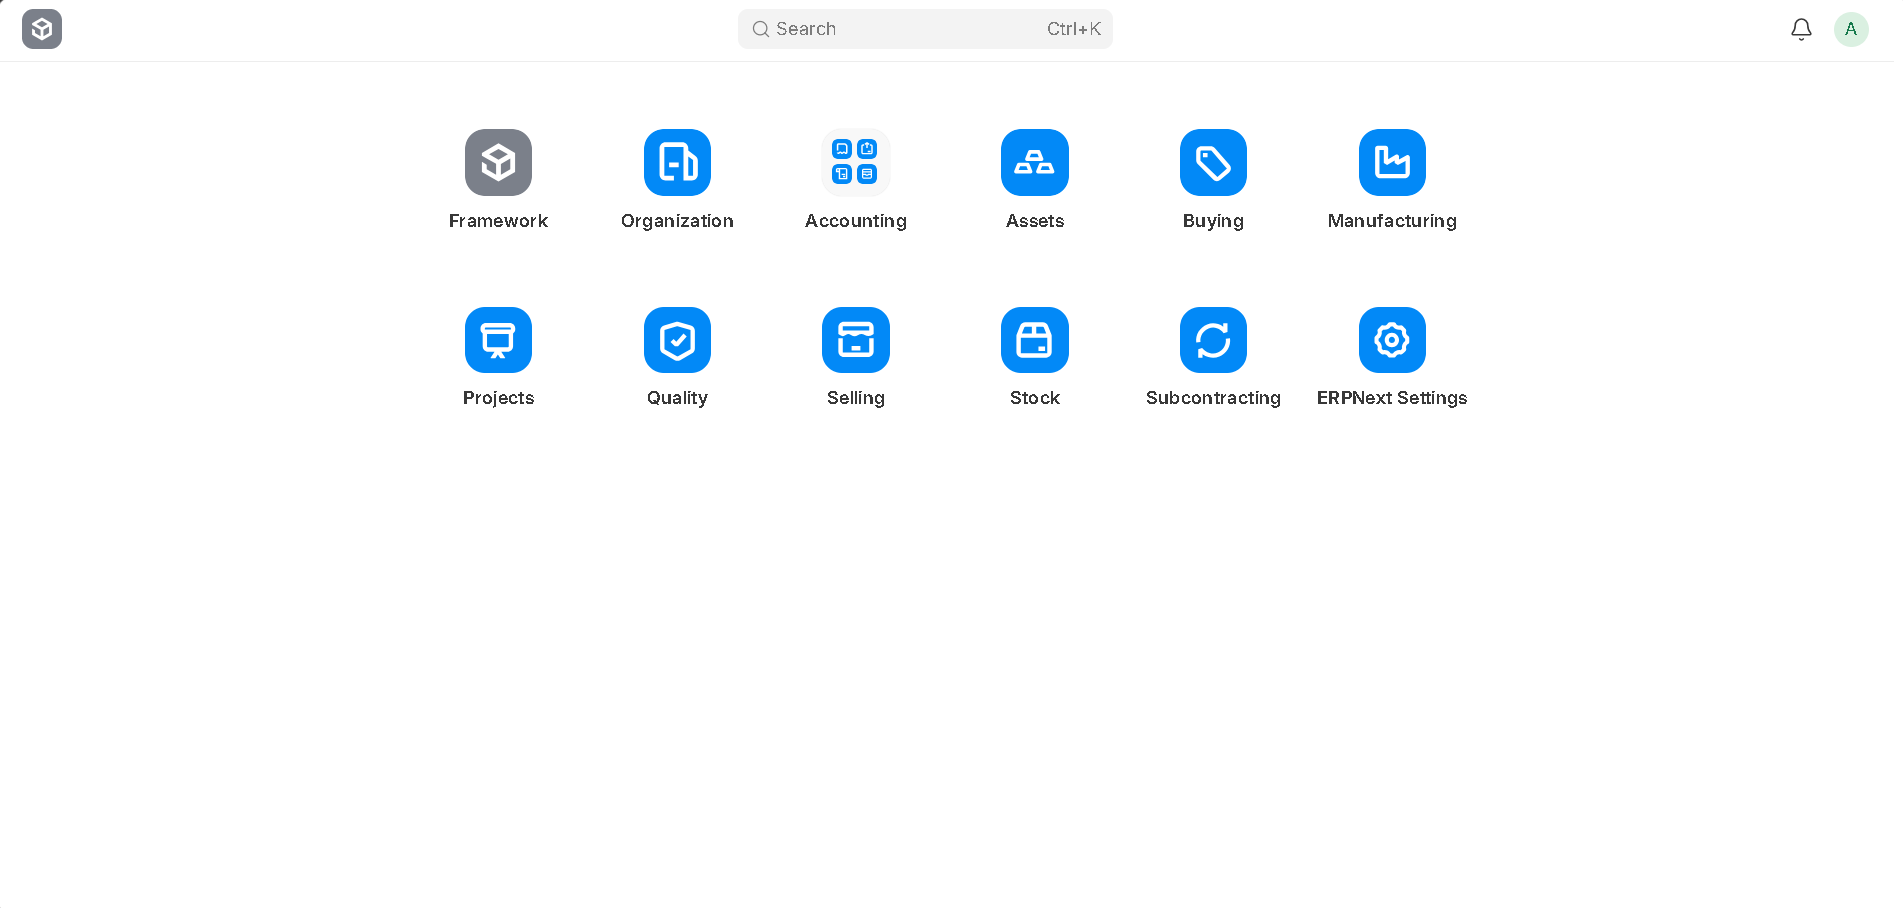
\includegraphics[width=1\linewidth]{images/erp.png}
        \caption{erp Logo}
        \label{fig:erp Logo}
    \end{figure}
    \begin{figure}[H]
        \centering
        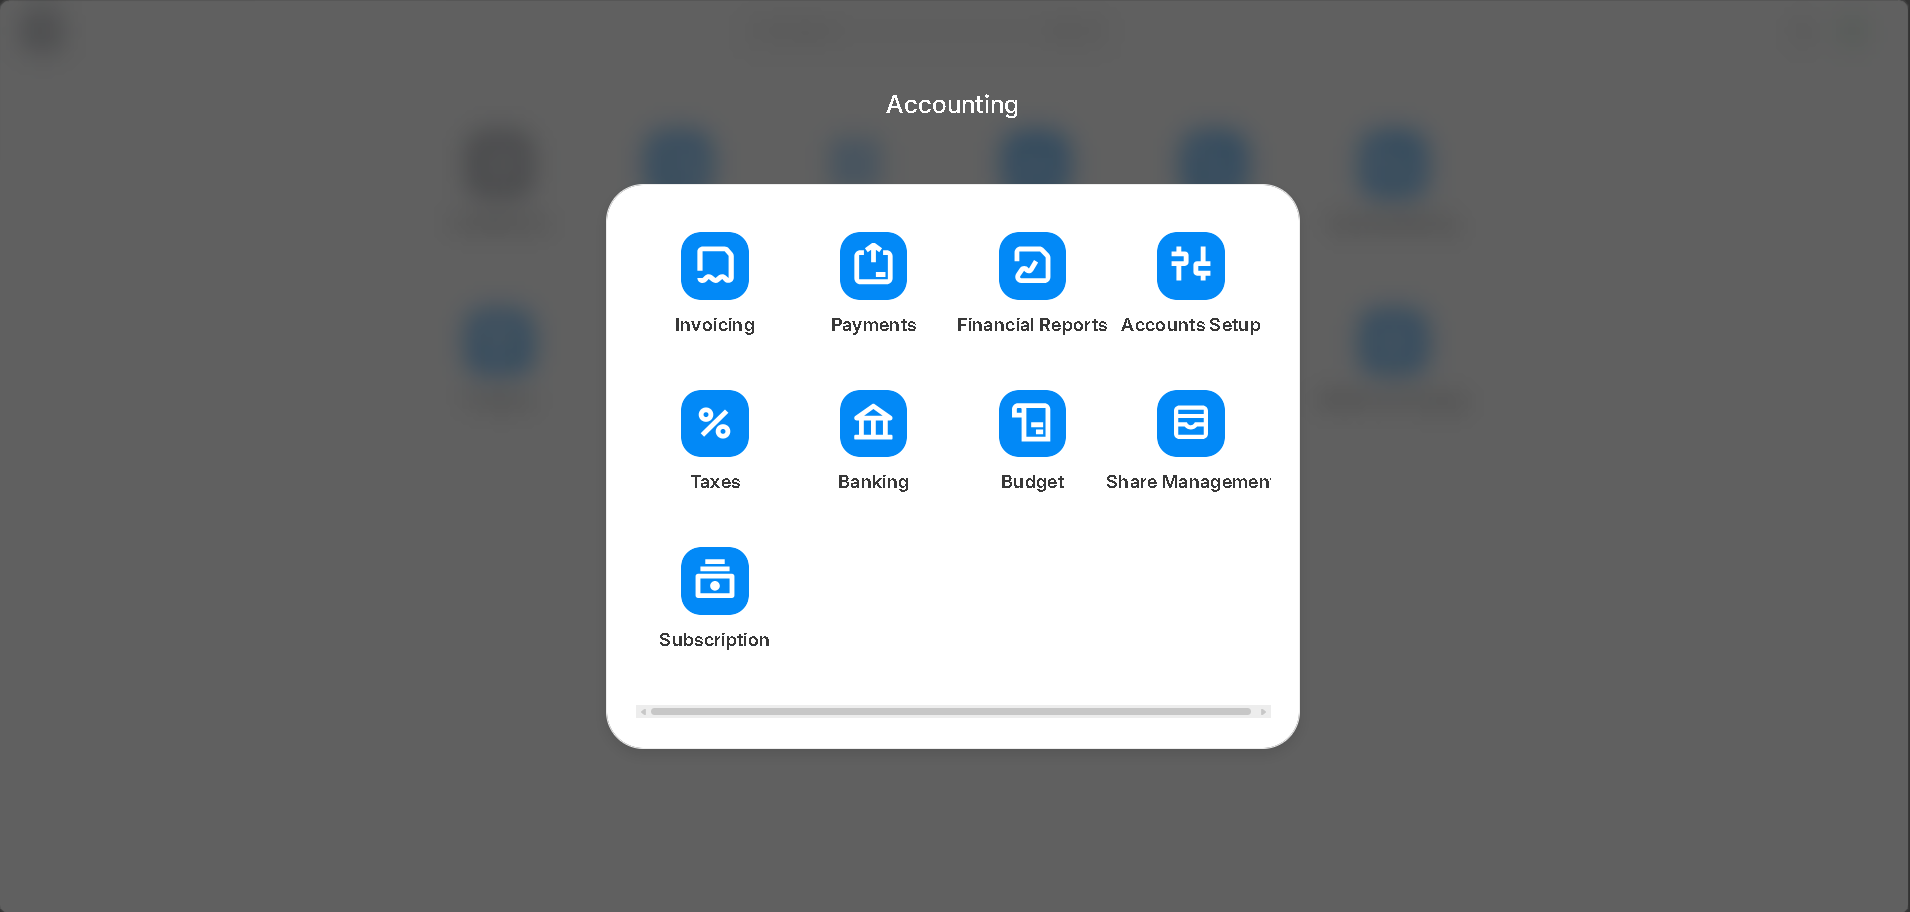
\includegraphics[width=1\linewidth]{images/erp_ext.png}
        \caption{erp-ext Logo}
        \label{fig:erp_ext Logo}
    \end{figure}
    \item \textbf{Dolibarr ERP \& CRM}:
    Dolibarr is a comprehensive web-based ERP and CRM tool aimed at small companies and freelancers. It offers billing, stock management, administrative records storage, and employee tracking features. It provides self-service client portals, but it is built on legacy web architectures and lacks a modern, reactive real-time mobile application for client-agency daily chat exchanges.
    \begin{figure}[H]
        \centering
        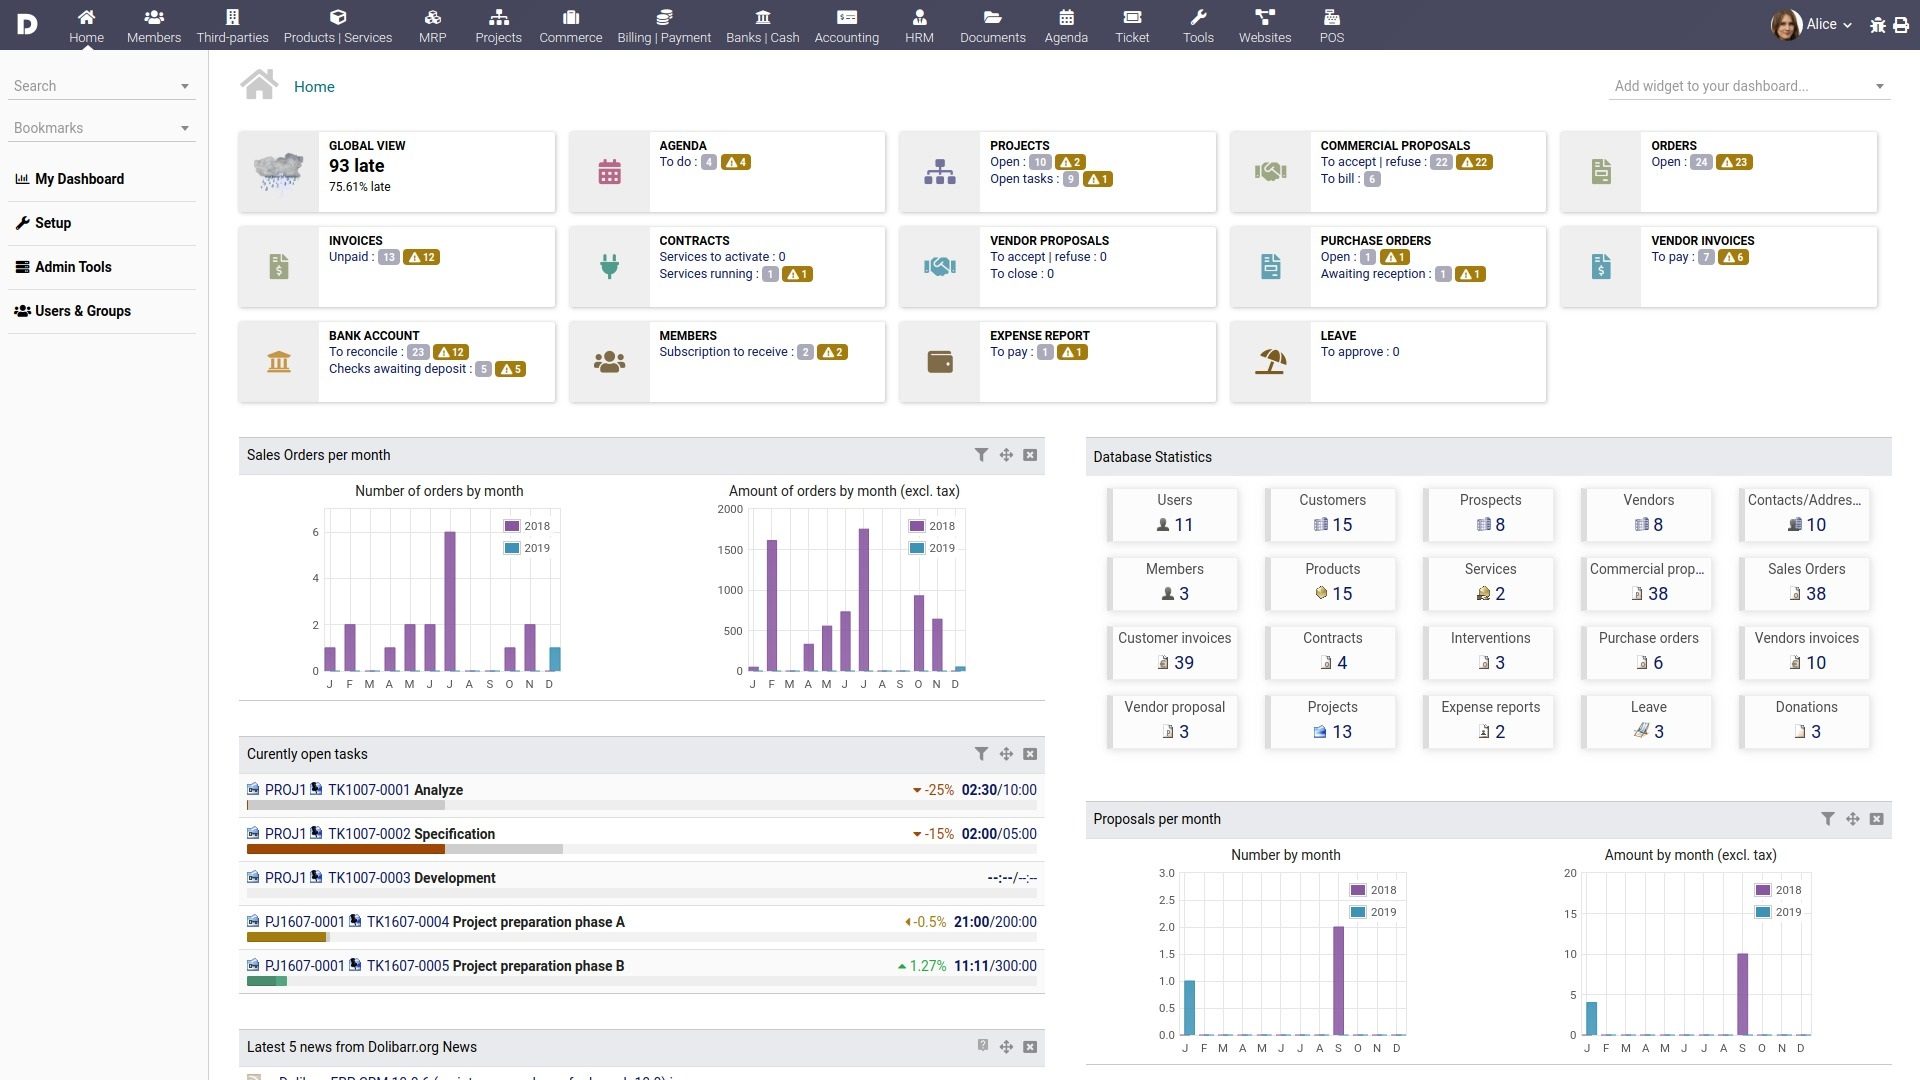
\includegraphics[width=1\linewidth]{images/dolibarr.jpg}
        \caption{Dolibarr Logo}
        \label{fig:Dolibarr Logo}
    \end{figure}
\end{itemize}
\vspace{-0.8cm}

\subsubsection{Comparison of the existing}
We studied the three systems from different aspects indicated in the table below:
\begin{table}[H]
\centering
\caption{Comparison between Odoo, ERPNext and Dolibarr}
\label{tab:comparison_existing}
\begin{tabular}{|l|p{3.8cm}|p{3.8cm}|p{3.8cm}|}
\hline
\textbf{Criteria} & \textbf{Odoo} & \textbf{ERPNext} & \textbf{Dolibarr} \\
\hline
\textbf{Target market} & Small to large businesses & Small to mid-size companies & Freelancers and SMEs \\
\hline
\textbf{Deployment} & On-premises or cloud & On-premises or cloud & On-premises or cloud \\
\hline
\textbf{Customization} & Highly customizable platform & Customizable via Frappe framework & Extensible via modules but layout is limited \\
\hline
\textbf{Document Sharing} & Full document management & File attachments in portal & Simple document storage per client \\
\hline
\textbf{Real-time Chat} & Yes, basic messaging & No native real-time chat & No native chat \\
\hline
\textbf{Mobile App} & Yes, responsive hybrid & Basic responsive view & Third-party apps only \\
\hline
\textbf{Open-source} & Yes (Community Edition) & Yes & Yes \\
\hline
\end{tabular}
\end{table}

\subsubsection{Criticism of the existing}
Based on the comparison of the existing systems, we note the following limitations:
\begin{itemize}
    \item \textbf{Odoo}: Although Odoo offers a wide range of features, it can be complex to learn and use. In addition, creating highly customized client portals or specific mobile functionalities often requires advanced customization or additional development efforts.
    \item \textbf{ERPNext}: While it simplifies document attachments and has a solid database schema, it lacks interactive real-time messaging workspaces where managers and client companies can communicate immediately.
    \item \textbf{Dolibarr}: Dolibarr is lightweight and free, but its interface is outdated and relies on legacy web technologies. It does not provide reactive, real-time feedback for document processing states or instant support messaging.
\end{itemize}

\subsubsection{Proposed solution}
To address the needs of HMI Stars Consulting and overcome the limitations of existing ERP solutions, we designed and developed a customized application ecosystem called \textbf{HMI Stars}.The solution consists of three main components:
\begin{enumerate}
    \item \textbf{A Web Application Platform:} Dedicated to HMI Stars Consulting managers, allowing them to register client companies, review uploaded files (categorized by type: KBIS, VAT, RIB, bank statements ...), and reply to client inquiries.
    \item \textbf{A Cross-Platform Mobile Application:} Dedicated to client managers, providing tools to manage their employees, log daily attendance, submit leave and absence requests, and upload documents.
    \item \textbf{A Real-Time Backend Server:} Powered by Supabase, handling instant synchronization of messages and files while guaranteeing strict data isolation using PostgreSQL Row Level Security (RLS).
\end{enumerate}

\subsubsection{Technology Choices}
The technical track of the project required selecting a cross-platform frontend framework and a backend-as-a-service platform. Table \ref{tab:tech_choices} summarizes the comparison criteria that guided our decisions.

\begin{table}[H]
\centering
\caption{Technology comparison for frontend framework and backend platform}
\label{tab:tech_choices}
\begin{tabular}{|l|p{5.5cm}|p{5.5cm}|}
\hline
\textbf{Criteria} & \textbf{Frontend Framework} & \textbf{Backend Platform} \\
\hline
\textbf{Options evaluated} & Flutter (Dart) vs. React Native (JavaScript) & Supabase (PostgreSQL) vs. Firebase (NoSQL) \\
\hline
\textbf{Single codebase} & Flutter compiles natively for Android, iOS, and Web from one Dart codebase & React Native requires separate web tooling (React Native Web) \\
\hline
\textbf{Data model} & -- & Supabase uses relational PostgreSQL tables with SQL joins; Firebase uses NoSQL document collections \\
\hline
\textbf{Row-level security} & -- & Supabase offers native PostgreSQL RLS policies; Firebase relies on Firestore security rules \\
\hline
\textbf{Real-time engine} & -- & Both provide real-time listeners; Supabase uses PostgreSQL change notifications over WebSockets \\
\hline
\textbf{Open-source} & Both are open-source & Supabase is fully open-source and self-hostable; Firebase is proprietary \\
\hline
\end{tabular}
\end{table}

We selected \textbf{Flutter} because it provides true cross-platform compilation from a single Dart codebase for mobile and web, which aligns with our requirement to build both a client mobile application and an administration web platform from a shared code structure. We selected \textbf{Supabase} over Firebase because the project's data model (companies, employees, contracts, attendance records) fits naturally into relational PostgreSQL tables with foreign key constraints and SQL joins. Additionally, Supabase's native Row Level Security (RLS) policies allow us to enforce strict per-company data isolation directly at the database level without additional application-layer logic.

\section{Methodological Choices and Work Organization}

\subsection{The Unified Process (2TUP)}

We chose the \textbf{2TUP (Two Track Unified Process)} methodology for the development of this project. This approach separates the development process into two parallel tracks: a \textbf{functional track}, focused on capturing business requirements, modeling use cases, and specifying system behavior; and a \textbf{technical track}, focused on selecting technologies, defining the architecture, and designing the database and deployment infrastructure. The two tracks converge during the Construction phase, where the functional specifications and technical decisions are merged into a working implementation.

Table \ref{tab:2tup_tracks} shows how the two tracks are distributed across the report chapters and sections.

\begin{table}[H]
\centering
\caption{Mapping of 2TUP tracks to report sections}
\label{tab:2tup_tracks}
\begin{tabular}{|l|p{5cm}|p{5cm}|}
\hline
\textbf{Phase} & \textbf{Functional Track} & \textbf{Technical Track} \\
\hline
Inception (Ch. 1 \& 2) & Use case diagrams, actor identification, priority table, detailed use case descriptions & Technology comparison (Flutter vs RN, Supabase vs Firebase) \\
\hline
Elaboration (Ch. 2) & Sequence diagrams, use case analysis, class diagram design & Non-functional requirements, architectural style selection, deployment architecture \\
\hline
Construction (Ch. 2) & Use case implementation mapping & Database mapping, implementation environment, subsystem identification, MVC pattern \\
\hline
Transition (Ch. 3) & Functional test cases, usability evaluation & Execution environment, deployment verification \\
\hline
\end{tabular}
\end{table}

Although the report presents both tracks within the same chapters for readability, each section addresses either the functional or the technical perspective. This adaptation was chosen because the project involves a small development team, where separating the tracks into entirely distinct documents would introduce unnecessary redundancy without adding clarity.

\subsubsection{Unified Modeling Language (UML)}
UML is used as the standard modeling language to specify, visualize, and document the different elements of the system throughout the functional development process.
\begin{figure}[H]
    \centering
    
\includegraphics[width=0.3\linewidth]{images/uml.png}
    \caption{UML}
    \label{fig:UML}
\end{figure}
\subsection{Work Organization}
The project timeline is organized around the four iterative phases of the Unified Process. Each phase targets specific deliverables and maps to a subset of the prioritized use cases. Table \ref{tab:iteration_schedule} presents the iteration schedule followed during the development of the HMI Stars system.

\begin{table}[H]
\centering
\caption{Project iteration schedule}
\label{tab:iteration_schedule}
\begin{tabular}{|l|l|p{4.5cm}|p{4cm}|}
\hline
\textbf{Phase} & \textbf{Duration} & \textbf{Key Deliverables} & \textbf{Use Cases Addressed} \\
\hline
Inception & 2 weeks & Requirements analysis, actor identification, use case diagrams, priority table & -- \\
\hline
Elaboration & 3 weeks & Architectural analysis, sequence diagrams, class diagram, database schema design & -- \\
\hline
Construction -- Iter. 1 & 3 weeks & Authentication module, employee CRUD, database mapping with RLS & UC-01, UC-02 \\
\hline
Construction -- Iter. 2 & 3 weeks & Attendance logging, leave request submission, offline caching & UC-03, UC-04 \\
\hline
Construction -- Iter. 3 & 3 weeks & Real-time chat, file upload, document management & UC-05, UC-06 \\
\hline
Construction -- Iter. 4 & 2 weeks & Warning templates, settings, document scanner, push notifications & UC-07, UC-08, UC-09 \\
\hline
Transition & 2 weeks & Functional testing, usability evaluation, deployment, report writing & -- \\
\hline
\end{tabular}
\end{table}


\section{Conclusion}
The study of the existing system highlights the urgent need to transition to a structured, secure communication platform. The 2TUP methodology provides a solid framework to develop this project. The next chapter will detail the design development, covering the Inception, Elaboration, and Construction phases.
